% This is samplepaper.tex, a sample chapter demonstrating the
% LLNCS macro package for Springer Computer Science proceedings;
% Version 2.20 of 2017/10/04
%
\documentclass[runningheads]{llncs}
%
\usepackage{graphicx}
% Used for displaying a sample figure. If possible, figure files should
% be included in EPS format.
%
% If you use the hyperref package, please uncomment the following line
% to display URLs in blue roman font according to Springer's eBook style:
% \renewcommand\UrlFont{\color{blue}\rmfamily}

\begin{document}
%
\title{A Shader-Based Architecture for Virtual Reality Applications on Mobile Devices\thanks{Supported by SIDIA}}
%
%\titlerunning{Abbreviated paper title}
% If the paper title is too long for the running head, you can set
% an abbreviated paper title here
%
\author{Adriano M. Gil \and
Thiago S. Figueira}
%
\authorrunning{F. Author et al.}
% First names are abbreviated in the running head.
% If there are more than two authors, 'et al.' is used.
%
\institute{SIDIA Instituto de Ci\^encia e Tecnologia, Manaus, Brazil
\email{\{adraino.gil\}@sidia.com}}
%
\maketitle              % typeset the header of the contribution
%
\begin{abstract}
The abstract should briefly summarize the contents of the paper in
150--250 words.

\keywords{First keyword  \and Second keyword \and Another keyword.}
\end{abstract}
%
%
%
\section{Introduction}

% TODO: Importance of VR
Virtual reality (VR) brings the promise of a revolution in the way entertainment is consumed in present times. The user is placed at the center of the action and perceives content from every direction.

% TODO: Performance issues games
Games, for their part, transport players to a world envisioned by game designers and developers. As the technology for other form factors such as PC and console advances, VR players want life-like graphics and improved responsiveness.

% TODO: Game architectures
Modern mainstream game consoles and PC sets allow parallel computing to be performed. In order to harness this extra computing power, it is necessary to move tasks from the single threaded game loop (figura 01) and place the ones that can run in parallel in different processors (figura 02).  

% TODO: Reasons/Motivation for a Shader-based architecture
VR devices, on the other hand, have a limited form factor. Issues like the heat generated by the processing components have to be taken into account which means adding more computing power is not possible without having side effects for the final user through the current form factor. The question is how to increase game performance using available components only?

% TODO: Importance of Unity
In VR games development, the most used game engine is \textit{Unity} and even though it is optimized, we believe there is an opportunity in exploring graphics cards for additional performance.

% TODO: Proposal
In this work, we propose an implementation of the classic game Snake using a shader-based architecture. By using a logic based of parallel execution we achieved a very performatic virtual reality application in which every visual element is defined and rendered by the shader in a unique mesh.

% TODO: Sections



\section{Related Work}

% TODO: Refs for VR Games, highlight performance/architecture concepts

% TODO: Refs for Games running only on GPU
The two-dimensional game \textit{GPGPUWars} \cite{joselli2009gpuwars} has its code structure based on \textit{shaders}, it is similar to the architecture presented here where the GPU performs all the processing of the game. However, applications in virtual reality differ from other applications because there is the need to fill the three-dimensional space to provide content for 3 degrees of freedom (3DoF-\textit{3 Degrees of Freedom}). For example, the application described in \cite{zund2015unfolding} uses computational vision to generate a panoramic view of an 8-bit console game.

% TODO: Refs for Games architectures

% TODO: Refs for GPU-based architectures


\section{VRSnake} \label{sec:vrsnake}
% TODO: Describe rules of the game
\textit{VRSnake} brings to virtual reality the classic 2D game \textit{Snake}, but unlike the original, the player controls the positioning of the collectible objects rather than directly controlling the snake. We propose the following rules:

\begin{enumerate}
\item The snake continuously and automatically seeks the collectible object and grows in a unit as it reaches this object;
\item The player sets the collectible object position;
\item The player wins when the \textit{snake} is defeated, that is, when it hits itself in some way.

\end{enumerate}

\section{Game architectures}

% TODO: What is a game architecture?
Games are a  software product, therefore the  architecture of a game is comparable to that of software and defines how the game is built. Usually, it is not apparent to the player, except for performance \cite{croft_2004}.

\begin{figure}
\caption{Simplified architecture of game engine according to \cite{portales}}
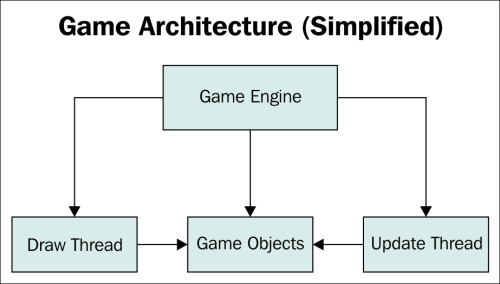
\includegraphics[scale=2, width=\textwidth]{src/hci2020-images/Game_Architecture_Raul_Portales.jpg}
\end{figure}

% TODO: Objectives of a game architecture?

\subsection{Game Loop architecture}

% Example of default game loop architectures

\subsection{Shader-based architecture}
 \label{subsec:shader-architecture}

% TODO: A general overview of a shader-based architecture
% TODO: What quality attributes/advantages we are seeking

We propose a the game architecture based on two layers: one layer is responsible for handling the logic of the game while the other is accountable for managing the rendering.  The logical layer controls intelligent tasks such as the search for the collectible objects and movement, furthermore, it is executed in the Central Processing Unit (CPU) in CSharp. The visualization layer involves a shader, a piece of code that runs directly in the Graphics Processing Unit (GPU), which is responsible for rendering all items displayed on the output device, which includes the collectible objects as well as the snake.

In other words, the logical layer manages the collision and movement of the snake as well as selects the most promising path given a randomization factor; The visualization layer, on the other hand, is responsible for rendering all the elements arranged in the output device, that is, the CPU has no influence over these objects.

\subsection{Proposed Architecture}

% Our proposal - Two layers
% Render layer
% Logic layer

\section{Render layer}

\subsection{Virtual reality in a inverted sphere}
The illusion in a virtual world and the consequent immersion sensation that comes with it requires visual material available from all possible angles as the \textit{gearVR} allows complete freedom of rotation, i.e. 3 degrees of Freedom (3DoF-\textit{3 degrees of Freedom}). Given that our proposal contemplates a 2D game, there is the challenge of displaying two-dimensional content in a 3D scenario so that everything happens around the user.

An inverted sphere, that is, a sphere that has only its inner side rendered, makes it possible to completely fill the entire field of view, it also is the standard solution adopted to display equirectangular images in 360 degrees. The procedural generation of a sphere can follow one of the two approaches below:

\begin{enumerate}
  \begin{item} An icosphere, i.e., a sphere which vertices are evenly distributed;
 \end{item}
  \begin{item} Generation of vertices based on longitude/latitude coordinates. \end{item}
\end{enumerate}

For this work, the second approach was adopted due to the possibility of using longitude/latitude as a way to map the UV coordinates through the equation below:

\begin{equation}
R^2 \leftarrow R^3 : (\lambda, \theta) \rightarrow (x, y, z)
\label{equation1}
\end{equation}

\subsection{Simple 2D Snakes}

\subsection{Raymarching Cube-based 3D Snakes}

\section{Logic layer}

\subsection{Managing Game Objects}

\subsection{Snake movement agent} \label{sec:agent}

The movement of the \textit{snake} is composed of a state evaluation function that analyzes each possible action at any given time. In essence, the serpent is always seeking  the collectible, so it evaluates the shortest distance course on the X and Y axes in the UV space and, provided that there is no possibility of hitting itself, takes this path and repeats the process. The function below illustrates this procedure:

\begin{equation}
F(A) = R * (D + O)
\label{equation11}
\end{equation}

Where \textit{R} is a randomization factor; \textit{D} represents the \textit{Manhattan} distance between the current position and the collectable object; And \textit{O} is a value attributed to the existence or not of obstacles in this path.

\section{Experiments and Results}

% TODO: Define metrics to evaluate architectures
% TODO: Experiment with normal game
% TODO: Experiment with shader-based game
% TODO: Experiment with VR shader-based game
% TODO: Experiment with shader-based game with Raymarching

\section{Conclusions}
We believe it is possible to explore the GPU for additional performance of virtual reality games in mobile devices. For the full paper, we intend to implement the game using the defined architecture and compare results using frames-per-second as the evaluation metric. We also see an opportunity for a full GPU implementation using ray-marching in a 3D environment.
%
% ---- Bibliography ----
%
% BibTeX users should specify bibliography style 'splncs04'.
% References will then be sorted and formatted in the correct style.
%
\bibliographystyle{splncs04}
\bibliography{shaderbasedarch}
\end{document}
